\documentclass[11pt,a4paper]{article}

\usepackage[margin=2.5cm]{geometry}
\usepackage[T1]{fontenc}
\usepackage{lmodern}
\usepackage{microtype}
\usepackage{amsmath}
\usepackage{booktabs}
\usepackage{graphicx}
\usepackage{xcolor}
\usepackage{tikz}
\usetikzlibrary{positioning,arrows.meta,calc}
\usepackage[hidelinks]{hyperref}

\title{\textbf{Spanner}: Domain-Adapted Extractive Question Answering with BERT}
\author{Piyush \and Nirdesh Gothania}
\date{}

\begin{document}
\maketitle

\begin{abstract}
We present \emph{Spanner}, a compact toolkit for extractive question answering (QA) over user-supplied documents. Given a question and a passage, the system predicts the start and end of the passage span that answers it. Spanner fine-tunes a BERT model, previously trained on SQuAD~2.0, on a small set of domain questions, and handles documents longer than the model's input limit with overlapping sliding windows. On a 17-question kangaroo knowledge set, domain fine-tuning raises Exact Match from 82.4 to 100.0. Every error made by the untuned model was a span-boundary mismatch, which fine-tuning corrected. The code, data and a command-line interface are available at \url{https://github.com/Anandpiyush21/spanner}.
\end{abstract}

\section{Introduction}

Extractive QA asks a model to locate the answer to a question inside a given passage, rather than generate free text. Because every answer is a substring of the source, the output can be traced back to the document and the model cannot invent facts. This makes it a good fit for question answering over manuals, notes and reference texts.

Pre-trained transformers such as BERT~\cite{devlin2019bert}, fine-tuned on large benchmarks like SQuAD~\cite{rajpurkar2016squad,rajpurkar2018know}, perform this task well on general text. A new domain, however, often has its own conventions for where an answer begins and ends. Spanner is a small, readable pipeline for adapting such a model to a domain with a few dozen examples, and then querying arbitrary documents from the command line.

\section{Method}

\subsection{Task formulation}

Let the question be $q$ and the context be a token sequence $c = (c_1, \dots, c_n)$. The model receives the pair as
\[
  \texttt{[CLS]}\; q \;\texttt{[SEP]}\; c \;\texttt{[SEP]}
\]
and produces, for every position $i$, a start logit $s_i$ and an end logit $e_i$ from a linear layer over BERT's final hidden states. These are normalised with a softmax over the context tokens to give $P_{\text{start}}(i)$ and $P_{\text{end}}(j)$.

\paragraph{Training.} Given gold token positions $(i^\ast, j^\ast)$, the loss is the mean of the two cross-entropies:
\[
  \mathcal{L} = -\tfrac{1}{2}\left(\log P_{\text{start}}(i^\ast) + \log P_{\text{end}}(j^\ast)\right).
\]

\paragraph{Inference.} The predicted answer is the highest-scoring valid span,
\[
  (\hat\imath, \hat\jmath) = \arg\max_{\substack{i \le j < i + L}} P_{\text{start}}(i)\, P_{\text{end}}(j),
\]
with maximum answer length $L = 30$ tokens. The span is mapped back to character offsets and sliced directly from the original text, which keeps its exact casing and punctuation.

\subsection{Aligning answers to tokens}

Annotations are given as character spans. We map them to token positions using the tokenizer's offset mapping, which records the character range covered by each token: $i^\ast$ is the first context token that ends after the answer starts, and $j^\ast$ is the last context token that begins before the answer ends. The data loader rejects any example whose answer is not an exact substring of its context, so labels can never point at text that is not there.

\subsection{Long documents}

BERT accepts at most 512 tokens, and we use windows of 384. A longer context is split into overlapping windows, each repeating the question, with a stride of 128 tokens shared between consecutive windows, so that no answer is lost at a boundary (Figure~\ref{fig:pipeline}). During training, a window that does not fully contain the answer is labelled with the \texttt{[CLS]} position, following the SQuAD~2.0 convention for ``no answer''. At inference, every window is scored and the best span across all windows is returned.

We implement the windowing ourselves rather than using the tokenizer's built-in overflow option, because \texttt{tokenizers}~0.23.x returns only a single overflow window for question--context pairs. The same function is used for training and inference, so both always see identical inputs.

\begin{figure}[t]
\centering
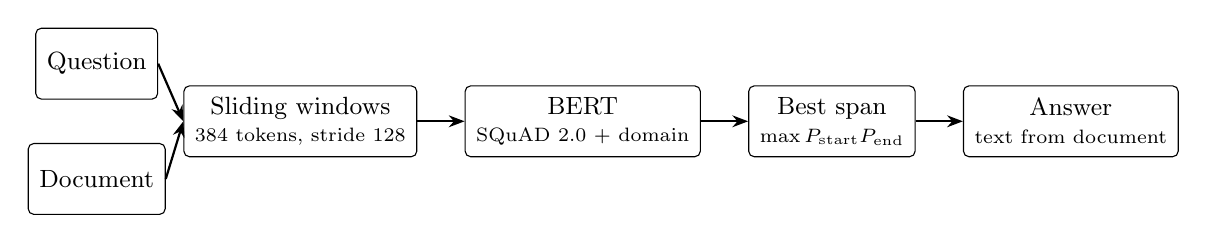
\begin{tikzpicture}[
  node distance=0.55cm and 0.6cm,
  box/.style={draw, rounded corners=2pt, align=center, font=\small, minimum height=0.9cm, inner sep=4pt},
  arr/.style={-{Stealth[length=2mm]}, thick}
]
  \node[box] (q) {Question};
  \node[box, below=of q] (c) {Document};
  \node[box, right=1.1cm of $(q)!0.5!(c)$] (w) {Sliding windows\\[-1pt]\scriptsize 384 tokens, stride 128};
  \node[box, right=of w] (b) {BERT\\[-1pt]\scriptsize SQuAD 2.0 + domain};
  \node[box, right=of b] (s) {Best span\\[-1pt]\scriptsize $\max P_{\text{start}} P_{\text{end}}$};
  \node[box, right=of s] (a) {Answer\\[-1pt]\scriptsize text from document};
  \draw[arr] (q.east) -- (w.west);
  \draw[arr] (c.east) -- (w.west);
  \draw[arr] (w) -- (b);
  \draw[arr] (b) -- (s);
  \draw[arr] (s) -- (a);
\end{tikzpicture}
\caption{The Spanner inference pipeline.}
\label{fig:pipeline}
\end{figure}

\section{Experimental setup}

\paragraph{Data.} The bundled dataset contains five passages about kangaroos (biology, behaviour, life cycle, ecology and conservation) with 17 questions in total, two to five per passage. Each answer is a short span copied verbatim from its passage. A separate, unannotated document, \texttt{kangaroo.txt}, is provided for interactive querying.

\paragraph{Model and training.} We start from \texttt{deepset/bert-base-uncased-squad2}, a BERT-base model (110M parameters) fine-tuned on SQuAD~2.0, loaded with the Hugging Face Transformers library~\cite{wolf2020transformers}. We train for 3 epochs with batch size 8 using AdamW~\cite{loshchilov2019adamw} (learning rate $3\times10^{-5}$, weight decay 0.01), a linear schedule with 10\% warmup, gradient clipping at 1.0, and seed 42. Training on a CPU takes about 90 seconds.

\paragraph{Metrics.} We report the standard SQuAD metrics~\cite{rajpurkar2016squad}. \emph{Exact Match} (EM) is the percentage of predictions identical to the gold answer after normalisation (lower-casing and removing punctuation and articles). \emph{F1} is the token-overlap F1 between prediction and gold answer, averaged over questions.

\section{Results}

\begin{table}[h]
\centering
\begin{tabular}{lcc}
\toprule
Model & EM & F1 \\
\midrule
SQuAD 2.0 BERT, no domain fine-tuning & 82.4 & 97.1 \\
+ 3 epochs on the kangaroo set (Spanner) & \textbf{100.0} & \textbf{100.0} \\
\bottomrule
\end{tabular}
\caption{Results on the 17-question kangaroo set.}
\label{tab:results}
\end{table}

The mean training loss fell from 0.234 in the first epoch to 0.158 and then 0.055. Table~\ref{tab:results} compares the model before and after fine-tuning.

\paragraph{Error analysis.} The untuned model's high F1 (97.1) shows that it already finds the right part of the passage. All three of its errors are boundary mismatches in which it omits a leading qualifier included in the gold answer:

\begin{center}
\small
\begin{tabular}{lll}
\toprule
Question & Predicted & Gold \\
\midrule
How fast can a red kangaroo run? & 56 kilometers per hour & \emph{up to} 56 kilometers per hour \\
How long do joeys nurse? & an extended period & \emph{for} an extended period \\
What does the digestive system allow? & extract nutrients \dots & \emph{efficiently} extract nutrients \dots \\
\bottomrule
\end{tabular}
\end{center}

Fine-tuning taught the model the annotation convention of this dataset: keep qualifying words such as \emph{up to} as part of the answer.

On the separate \texttt{kangaroo.txt} document, which paraphrases the training passages, the fine-tuned model answers questions such as \emph{``What do kangaroos eat?''} with \emph{``grasses and other vegetation''} (confidence 0.98) and \emph{``Where do female kangaroos nurture their young?''} with \emph{``in a specialized pouch''} (0.98).

\section{Limitations and future work}

The scores in Table~\ref{tab:results} are measured on the training questions, so they show that the model fits the domain's conventions, not that it generalises to new questions. A held-out test set, ideally with several reference answers per question, is needed to measure generalisation. The dataset is also very small and covers a single topic. Natural next steps are to evaluate on a held-out split, to use the ``no answer'' option of SQuAD~2.0 so the system can decline unanswerable questions, and to add a retrieval stage so that questions can be asked over many documents at once.

\section{Conclusion}

Spanner shows that a SQuAD-trained BERT model can be adapted to a new domain's answer conventions with only a handful of examples, provided the training labels are aligned precisely to tokens. Together with sliding-window inference over long documents, this gives a small and reliable way to ask questions about one's own text.

{\small
\begin{thebibliography}{9}
\setlength{\itemsep}{1pt}
\bibitem{devlin2019bert}
J.~Devlin, M.-W.~Chang, K.~Lee, and K.~Toutanova.
BERT: Pre-training of deep bidirectional transformers for language understanding.
In \emph{Proceedings of NAACL-HLT}, 2019.

\bibitem{rajpurkar2016squad}
P.~Rajpurkar, J.~Zhang, K.~Lopyrev, and P.~Liang.
SQuAD: 100,000+ questions for machine comprehension of text.
In \emph{Proceedings of EMNLP}, 2016.

\bibitem{rajpurkar2018know}
P.~Rajpurkar, R.~Jia, and P.~Liang.
Know what you don't know: Unanswerable questions for SQuAD.
In \emph{Proceedings of ACL}, 2018.

\bibitem{wolf2020transformers}
T.~Wolf et~al.
Transformers: State-of-the-art natural language processing.
In \emph{Proceedings of EMNLP: System Demonstrations}, 2020.

\bibitem{loshchilov2019adamw}
I.~Loshchilov and F.~Hutter.
Decoupled weight decay regularization.
In \emph{Proceedings of ICLR}, 2019.
\end{thebibliography}
}

\end{document}
